% You should title the file with a .tex extension (hw1.tex, for example)
\documentclass[11pt]{article}

\usepackage{amsmath}
\usepackage{mathtools}
\usepackage{amssymb}
\usepackage{wrapfig}
\usepackage{fancyhdr}
\usepackage{tikz-qtree}
\usepackage{tikz-qtree-compat}
\usepackage[normalem]{ulem}
\usepackage{tikz}
\usepackage{graphicx}
\usepackage{lineno}
\DeclareMathOperator*{\argmin}{argmin}
\DeclareMathOperator*{\argmax}{argmax}

\oddsidemargin0cm
\topmargin-2cm     %I recommend adding these three lines to increase the 
\textwidth16.5cm   %amount of usable space on the page (and save trees)
\textheight23.5cm  

\newcommand{\question}[2] {\vspace{.25in} \hrule\vspace{0.5em}
\noindent{\bf #1: #2} \vspace{0.5em}
\hrule \vspace{.10in}}
\renewcommand{\part}[1] {\vspace{.10in} {\bf (#1)}}
\linespread{1.5}

\newcommand{\myname}{Anonymous Authors}
\newcommand{\myhwnum}{12}

\setlength{\parindent}{0pt}
\setlength{\parskip}{5pt plus 1pt}
 
\DeclarePairedDelimiter\abs{\lvert}{\rvert}%

\pagestyle{fancyplain}

\begin{document}
\medskip                        % Skip a "medium" amount of space
                                % (latex determines what medium is)
                                % Also try: \bigskip, \littleskip

\thispagestyle{plain}
{\Large Interrogating theoretical models of computation with deep learning} \\
Sean R. Bittner, Agostina Palmigiano, Alex T. Piet, Chunyu A. Duan, Francesca Mastrogiuseppe, Srdjan Ostojic, Carlos D. Brody, Kenneth D. Miller, and John P. Cunningham.

\linenumbers
\section{Abstract}
The cornerstone of theoretical neuroscience is the circuit model: a system of equations that capture a hypothesized neural mechanism of scientific importance.  At its best, such a model will give rise to an experimentally observed phenomenon -- whether behavioral or in terms of neural activity -- and thus can offer insight into neural computation.  The behavior of these circuits, like all models, critically depends on the choices of model parameters.  Historically, the gold standard has been to analytically derive the relationship between model parameters and emergent properties of computation.  However, this enterprise quickly becomes infeasible as biologically realistic constraints are included into the model, resulting often in \emph{ad hoc} approaches to understanding the relationship between model and computation.  Here we advance cutting edge machine learning -- the use of deep learning for probabilistic inference -- to learn parameter distributions that produce the emergent properties of computation.   Importantly, the techniques we introduce offer a logical and unbiased means to understand the implications of model parameter choices on scientific properties of interest.  To make these contributions concrete, we use these techniques to discover novel insights into network syncing in the stomatogastric ganglion, neuron-type input-responsivity in primary visual cortex, rapid task switching in superior colliculus, and approximate Bayesian inference in recurrent neural networks. More generally, this work inspires a shift of focus in theoretical neuroscience away from the historical gold standard. Let's forgo derivations when they are impossible, and leverage the modern inference engine to focus on understanding biologically relevant models.
%(150 word limit) we can ignore that for now up to about 50% \\

\section{Introduction}

The fundamental purpose of theoretical neuroscience is to use a mathematical \emph{model} to understand neural computation, whether that computation enables perception, action, or some intermediate calculation or processing \cite{abbott2008theoretical}.  
A theory of a neural computation is systematized with a set of equations -- the model -- and these equations are motivated by biophysics, neurophysiology, and/or other conceptual considerations.
The function of this system is governed by the choice of model parameters, which when configured \emph{just so}, give rise to some measurable signature of a computation.   
The work of analyzing a model then becomes the inverse problem: given a computation of interest, how can we reason about the parameters -- their likely values, their degeneracies, their attractor states and phase transitions, etc?  
For concreteness, consider the idealized practice: a theorist considers a model carefully and analytically derives how model parameters govern the computation.  
Celebrated examples of this gold standard include our field's understanding of memory capacity in associative neural networks \cite{hopfield1984neurons}, chaos and autocorrelation timescales in random neural networks \cite{sompolinsky1988chaos}, and the paradoxical effect in excitatory/inhibitory networks \cite{tsodyks1997paradoxical}.  

Unfortunately, as circuit models include more biological realism, theory via analytic derivation becomes infeasible.  
This fact creates an unfavorable tradeoff for the theorist.  On the one hand, one may tractably analyze systems of equations with unrealistic assumptions (for example symmetry or gaussianity), producing accurate inferences about parameters of a too-simple model.  On the other hand, one may choose a more biologically relevant model at the cost of \emph{ad hoc} approaches to analysis, producing questionable or partial inferences about parameters of an appropriately complex (and one presumes, scientifically interesting) model.  % intentionally belaboring the "inference about model parameters" to set the mindset of what *the* important question is.

% now transition to ML...
In parallel, this same tradeoff has been confronted in many scientific fields, with notable response from the machine learning community.  %it's timely and it's important, we're bringing these tools together...
% large scale inference engines exist, but maybe not in that language.  Of course ML has been very active in neuro, indeed with deep models also. 

% now our problem.  

Classically, statistical inference is a formalized way of describing the probabilistic relationship between observed data and model parameters.  However, statistical inference is impracticable in neural system models, because the likelihood functions are generally intractable.  Research in neural data analysis, which has enhanced our knowledge of a[kass], b[brown], c[paninski], d[jpcunni], e[pillow], focuses on the development of statistically inferable models for neural data sets, where such likelihood functions are tractable. Likelihood function intractability thus creates a gap between the models analyzed by theoreticians (motivated by laws of nature and physiology) and the probabilistic models developed by neural data scientists (constrained by tractability of inference) (Figure 1?).   Theoretical neuroscientists are careful about model creation, where neural data analysts are practical.  Neural data analysts are careful about inference of model parameters, where theoretical neuroscientists are practical.  This motivates the question: can we start doing \emph{careful} inference in \emph{careful} models? \\

\begin{figure}
\begin{center}
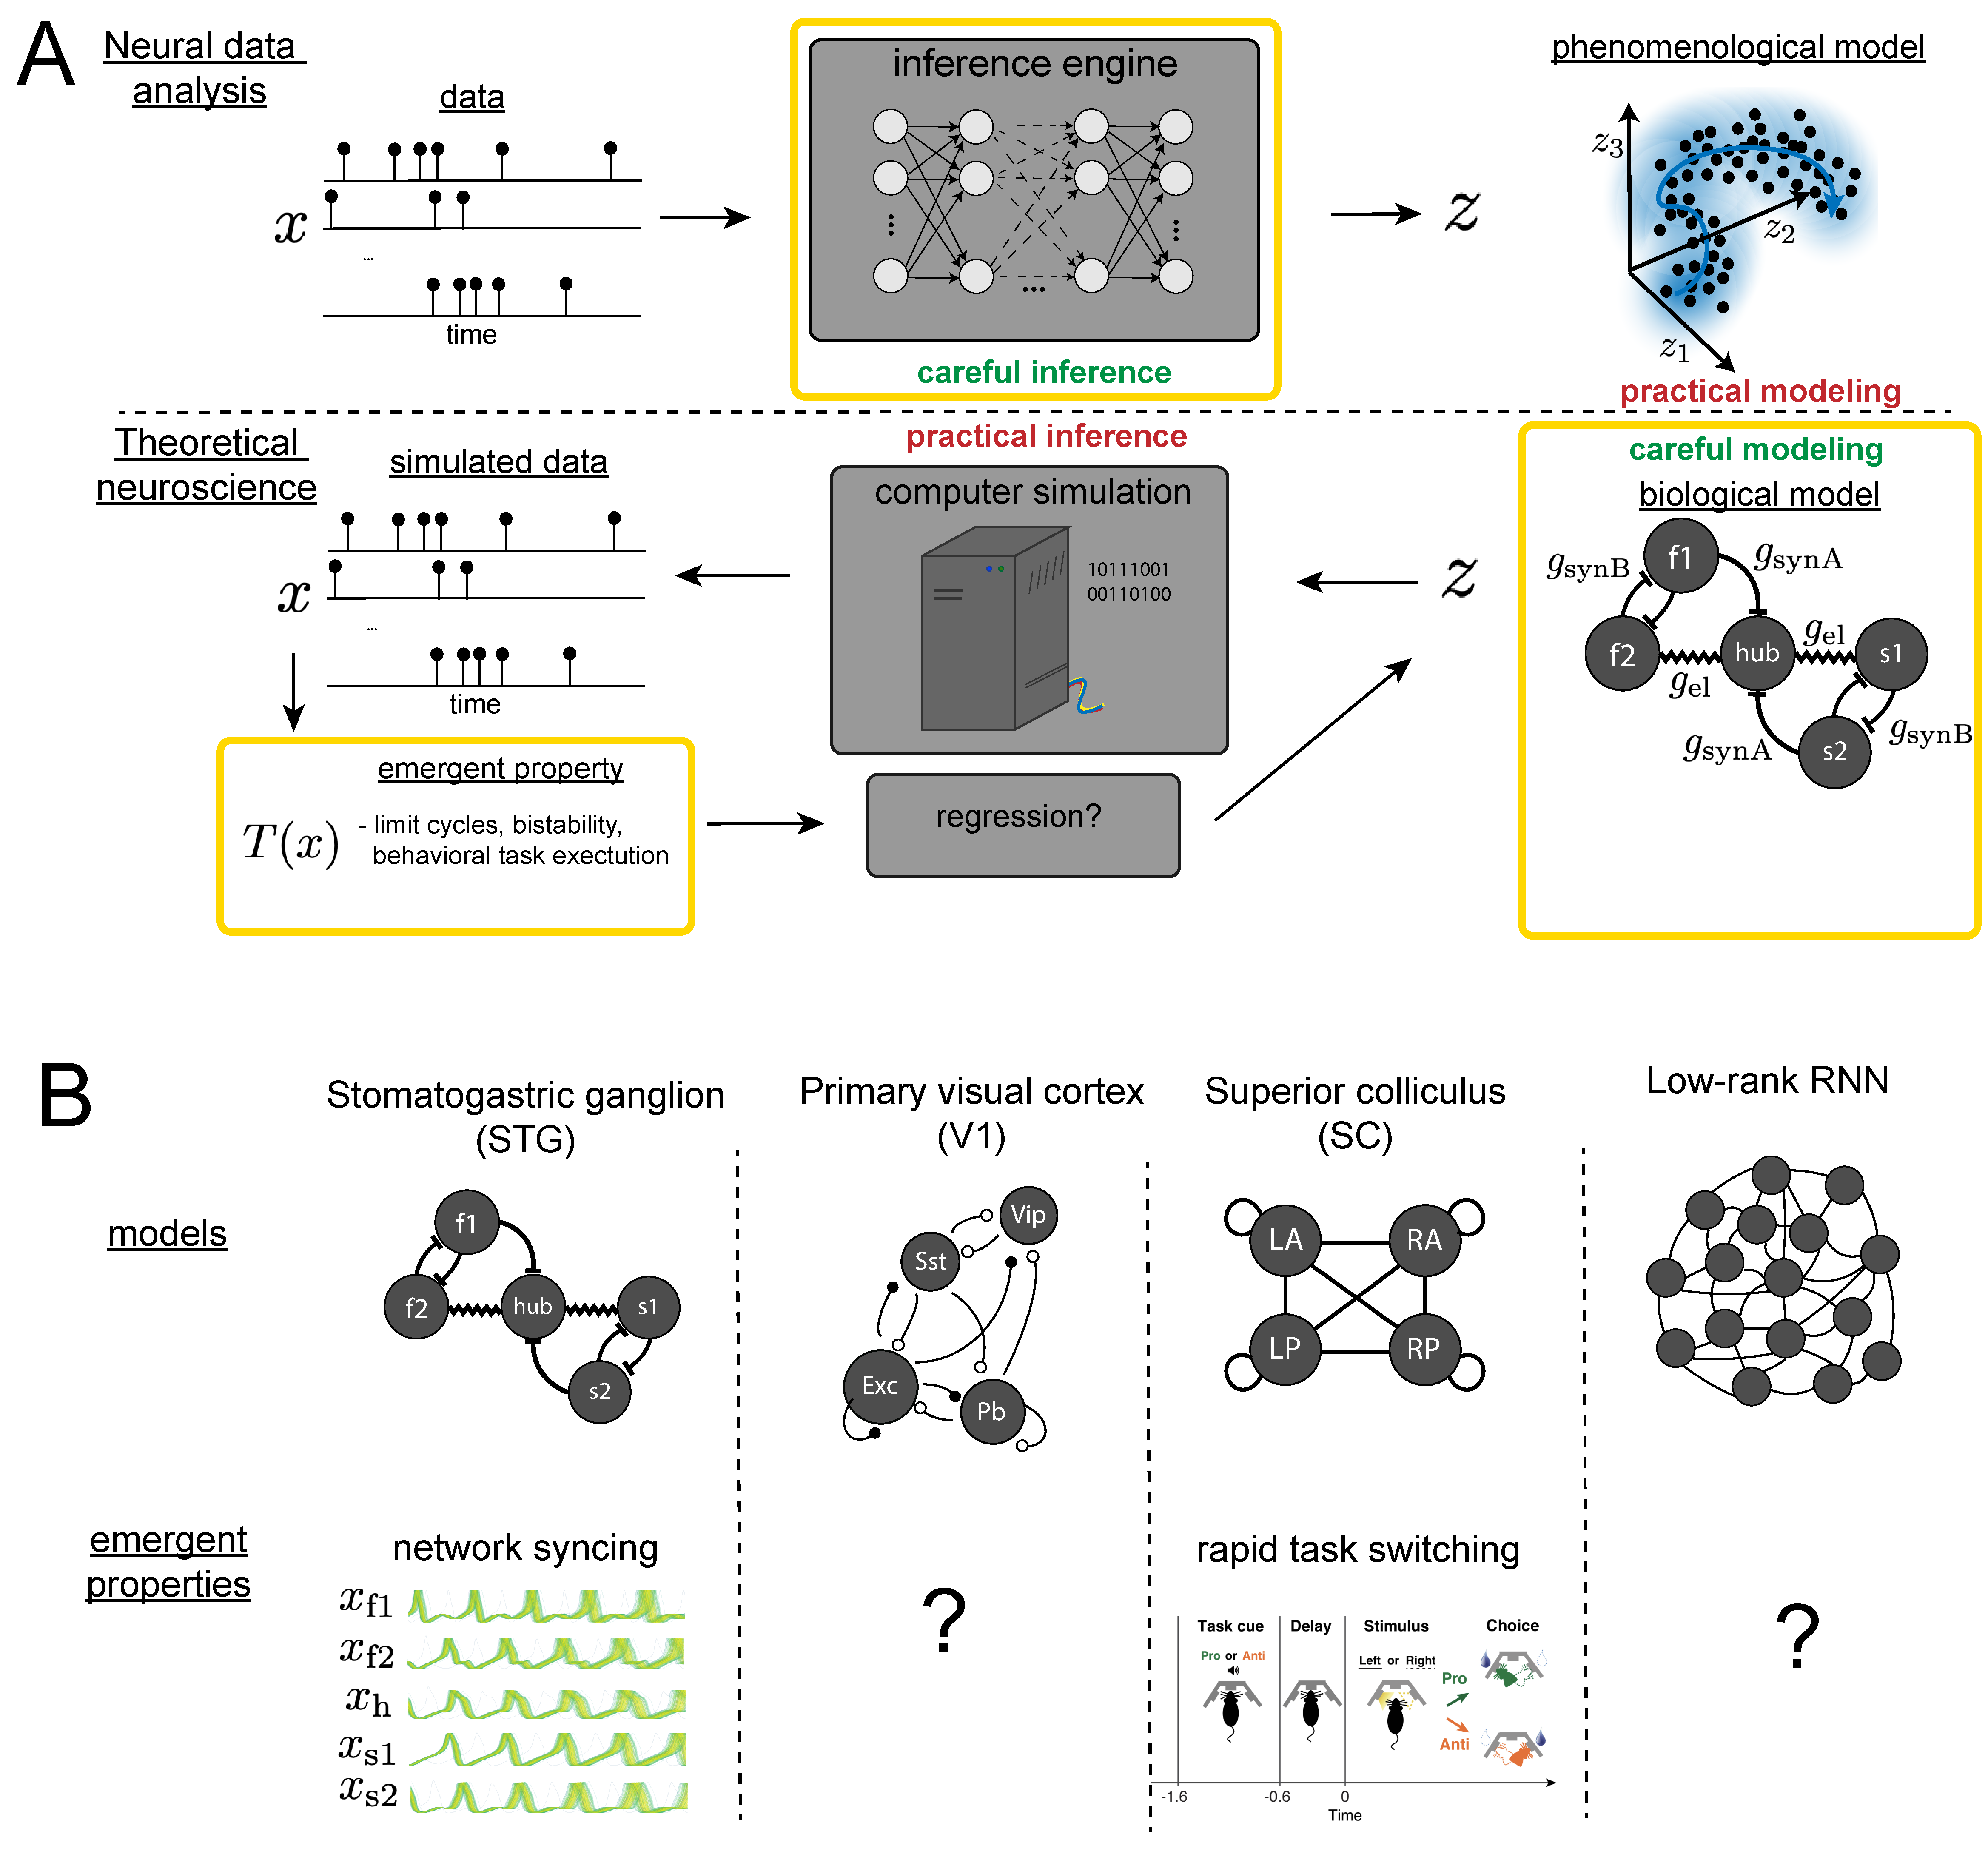
\includegraphics[scale=0.2]{figs/fig1/fig1.pdf}
\end{center}
\caption{\small A. \textit{Neural data analysis}: To identify structure in experimentally recorded neural data sets (left), neural data analysts use the modern inference engine (center) -- a collection of tools like convex optimization theory and deep learning from the machine learning literature -- to carefully execute Bayesian inference on a phenomenological generative model of the data.  Neural data analysts impose practical constraints to these phenomenological models so that Bayesian inference can be done. \textit{Theoretical Neuroscience}: Theoretical neuroscientists design systems of equations reflecting biological reality comprising a model (right, e.g. the STG) with the hopes of reproducing emergent properties of neural computation found in data (left).  In standard practice, models are evaluated by simulating them for many choices of parameters on a server (center).  To gain an understanding for how parameters of the model govern such emergent properties, theoretical neuroscientists are left to measure correlations or find other structure in the simulated activity. In this study, we introduce DSNs, which use the modern inference engine to learn distributions of model solutions given emergent properties of neural computations (yellow boxes).  B. We use DSNs to provide novel insights to popular models in theoretical neuroscience.  We examine network syncing in the STG, blah in a dynamic four neuron-type population model of primary visual cortex (V1), information routing in the superior colliculus (SC), and blah in low-rank recurrent neural networks (RNNs).}
\end{figure}


Advancements in probabilistic machine learning have led to transformative changes in industrial applications like image processing (sparse cite), speech recognition (sparse cite), text classification (sparse cite), and more.  We call the generalizable components of this groundbreaking technology (deep learning, stochastic gradient descent, GPU parallelization, etc.) the ``modern inference engine." (Point to work from Cunningham/Paninski using modern inference engine for neuroscientific phenomenological models (PfLDS, BehaveNET)?) In this study, we use the modern inference engine to bypass the perceived intractability of statistical inference in realistic models of neural systems.  (Introduce SDNs?)  We demonstrate the widespread applicability of this approach by producing novel insights into network syncing in the stomatogastric ganglion (STG), neuron-type input-responsivity in primary visual cortex (V1), rapid task switching in superior colliculus (SC), and approximate Bayesian inference in recurrent neural networks (RNNs). \\

\section{Results}
\subsection{Degenerate solution networks}
\begin{itemize}
\item To translate progress in neural data analysis to theoretical neuro, need to key steps.
\begin{itemize}
\item 1. Need to learn parameter distributions of biologically realistic (not just phenom.) models.
\item 2. Must be able to condition on emergent properties of interest, not simply computationally convenient sufficient statistics of data sets.
\end{itemize}
\item Bayesian data scientists will say experimental data is all that matters.  
\item \textit{Transition}: This is untrue when working in a creative, exploratory modeling setting.
\end{itemize}

\textbf{Edgy contrarian point about theorists and data}
\begin{itemize}
\item Common misconception: theoreticians rarely attempt to directly reproduce experimental data. 
\item Instead, they work with (abstracted?) mathematical definitions of emergent properties.  
\end{itemize}

\textbf{DSNs}
\begin{itemize}
\item We introduce DSNs, which bridge methodology in these subfields of comp neuro.
\item  Combine ideas from MEFNs (cite Gabe) and LFVI (cite Dustin) to learn a deep probability distribution of theoretical model parameterizations $z$ that produce the emergent properties of interest $T(x)$ (see Appendix).  
\item Explain deep probability distributions.
\item DSNs are deep probability distributions of theoretical model parameters, which are optimized to be maximally random (maximum entropy) while producing the specified value of emergent properties:
\begin{equation}
\begin{split}
q_\theta^*(z) &= \argmax_{q_\theta \in Q} H(q_\theta(z)) \\
 &  \text{s.t.  } E_{z \sim q_\theta}\left[ E_{x\sim p(x \mid z)}\left[T(x)\right] \right] = \mu \\
 \end{split}
\end{equation}
\end{itemize}

\begin{figure}
\begin{center}
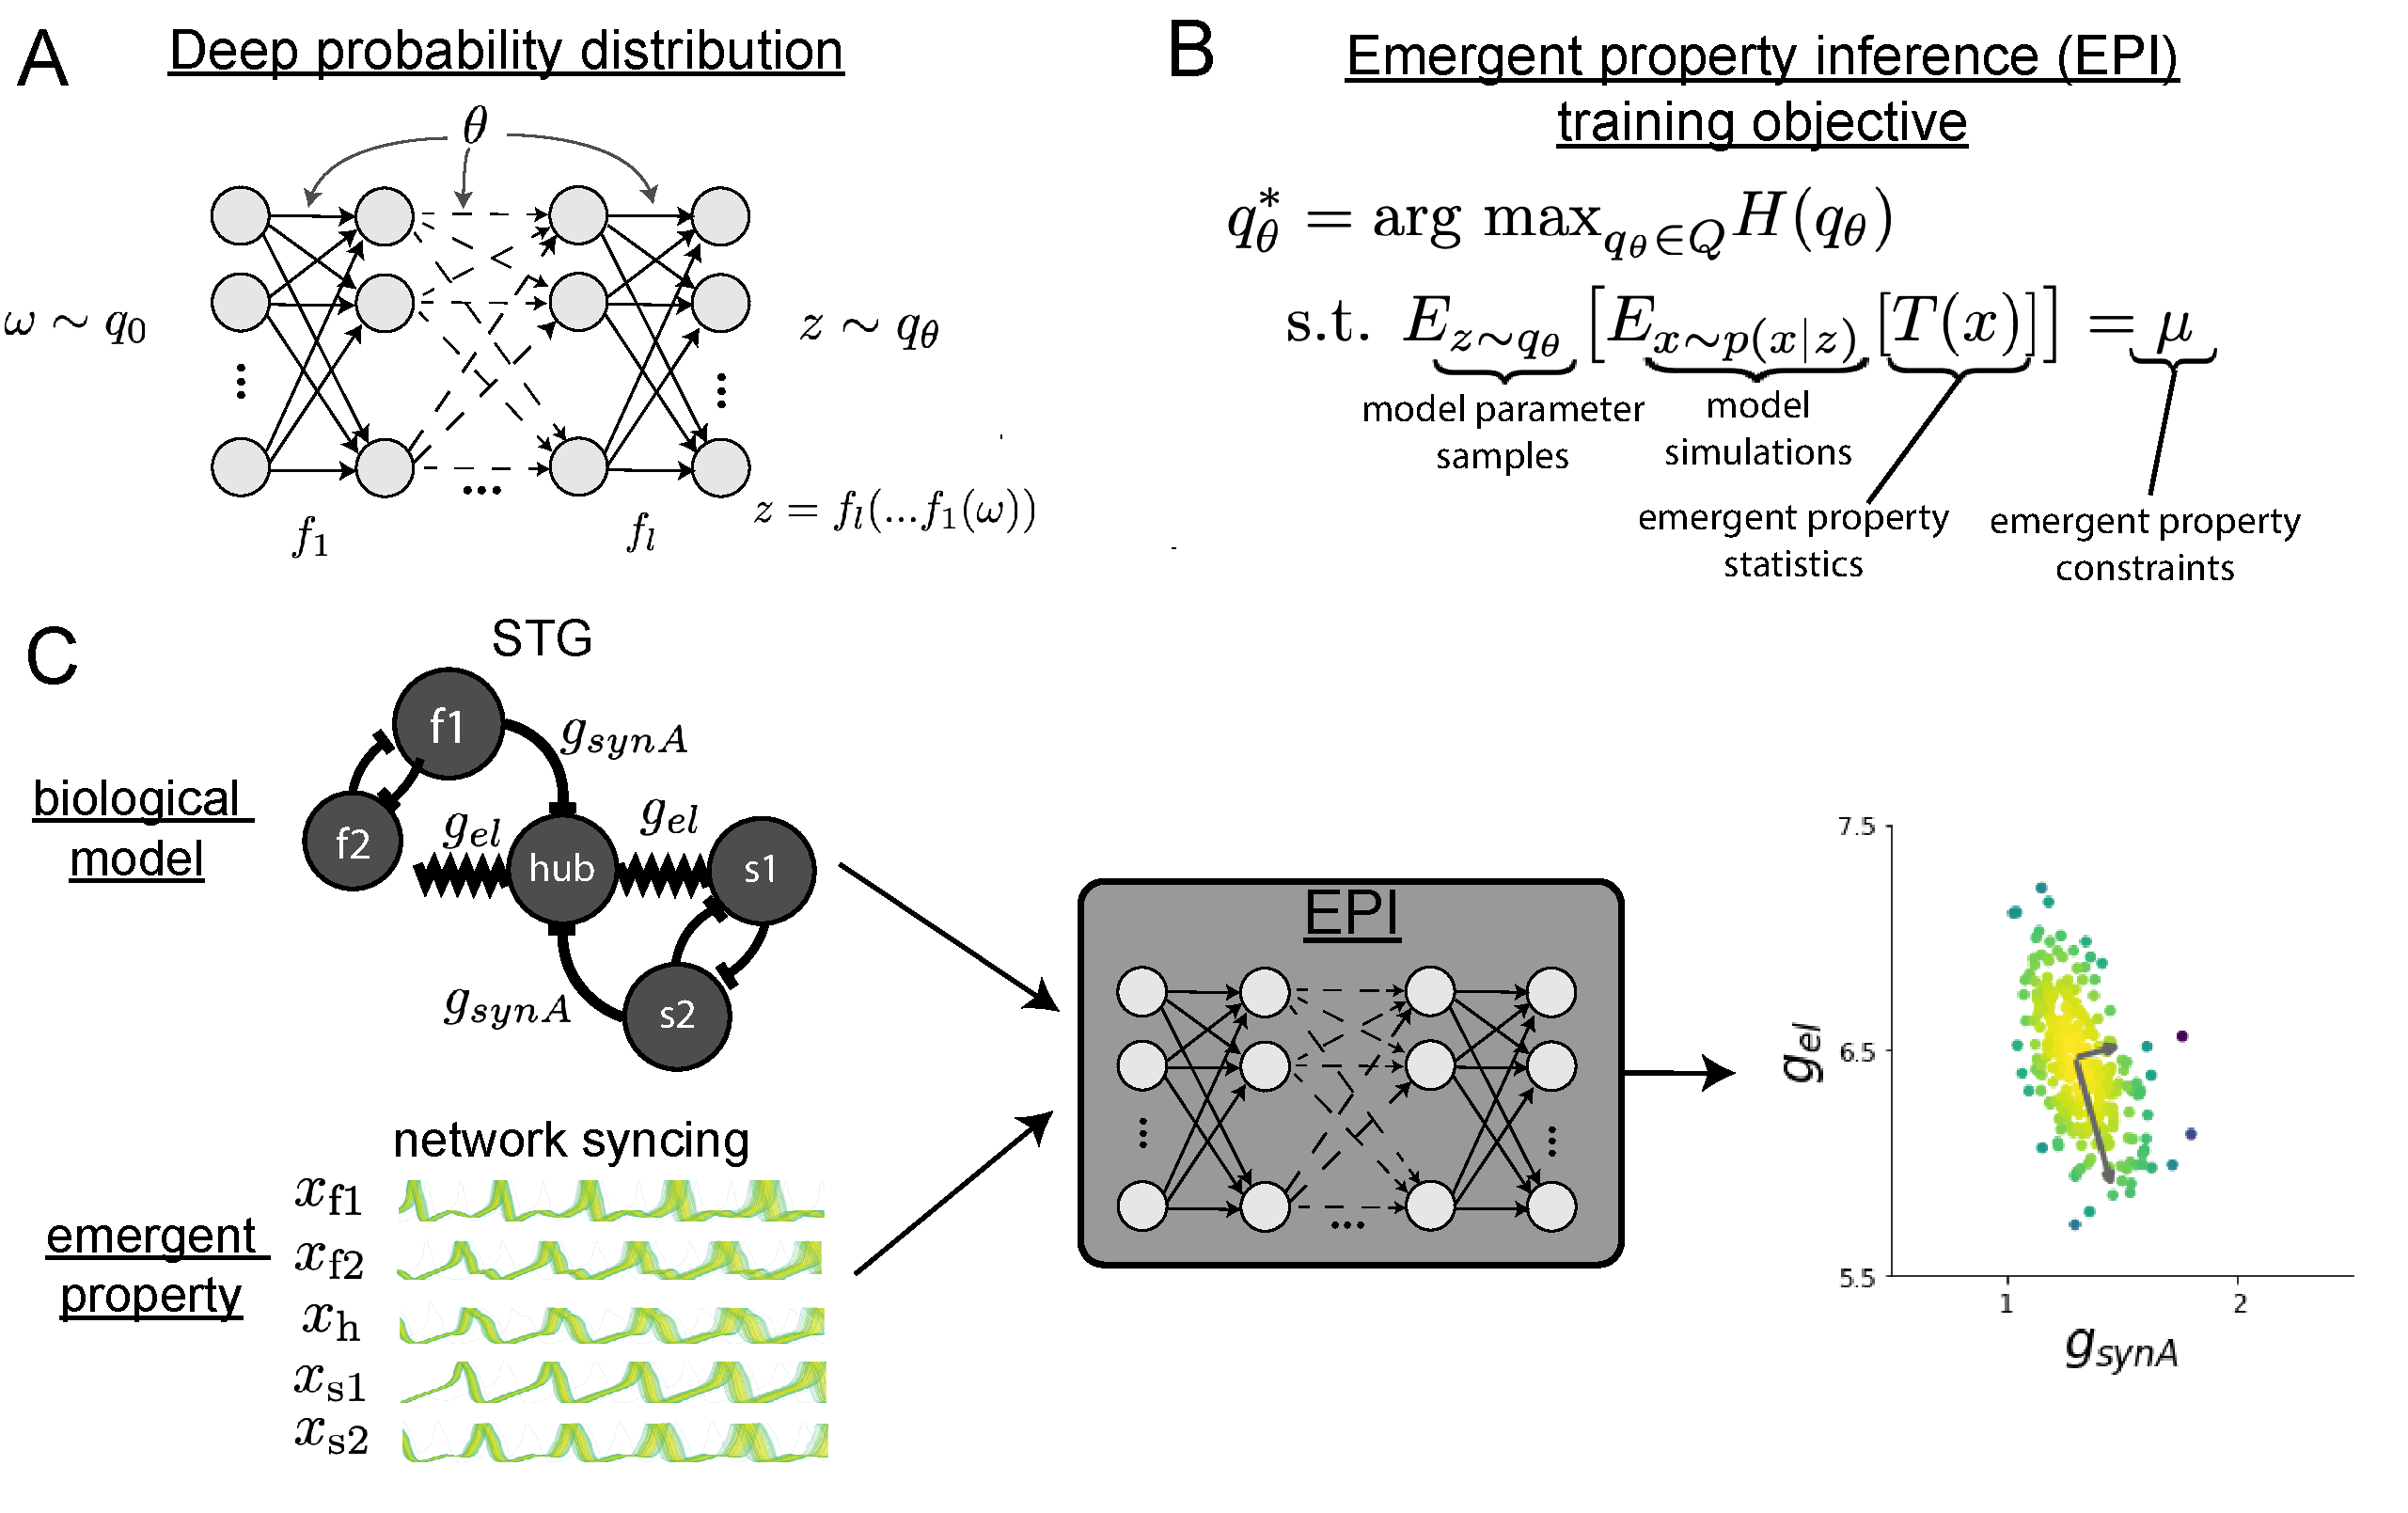
\includegraphics[scale=0.4]{figs/fig2/fig2.pdf}
\end{center}
\caption{A. Degenerate solution networks (DSNs) are deep probability distributions $q_\theta(z)$ of theoretical model parameterizations that produce emergent properties of interest.  The stochasticity of a deep probability distribution comes from a simple random variable $\omega \sim q_0$, where $q_0$ is often chosen to be an isotropic gaussian, and the structure comes from the deterministic transformation made by the deep neural network with optimized parameters $\theta$.  DSNs are the result of a constrained stochastic optimization, in which emergent properties $T(x)$ are fixed in expectation over model simulations $x \sim p(x \mid z)$ and DSN samples $z \sim q_\theta(z)$ to be a particular value $\mu$.  DSNs distributions maximize randomness through entropy. B. For a choice of model (STG) and emergent property (network syncing), a DSN learns a posterior distribution of the model parameters  $z = \left[g_{\text{el}}, g_{\text{synA}} \right]^\top$ conditioned on network syncing.}
\textbf{SB Comment}: In A, we have gaussian noise being fed into the deep probability distribution, and in B, we have a choice of model and emergent property predicating what the DSN is going to do.  There should be a way to depict these ideas without creating confusion on what the input to the DSN is.
\end{figure}

\textbf{Worked example: STG}
\begin{itemize}
\item For example, consider the STG.
\item Explain this STG circuit, emergent property of interest.
\item  For our choices of STG as model and network syncing as emergent property, we use a DSN to learn a distribution on STG conductance parameters that produces network syncing.  
\item Emphasize utility of DSN using Hessian.
\item An equivalent conceptualization is that DSNs do Bayesian inference (see Appendix).
\item Punchline about DSNs and transition to V1.
\end{itemize}

\subsection{Exploratory analysis of a theoretical model}
Will focus on this once result finalized.  Have a lot of text to pull from.

\subsection{Identifying sufficient mechanisms of task learning}
Will focus on this once V1 and LRRNN finalized.  Have a lot of text to pull from.

\subsection{Conditioning on computation with interpretable models of RNNs}
Will focus on this once result finalized.  Have a lot of text to pull from.

\section{Discussion}
\begin{itemize}
\item Summarize the key methodlogical demonstrations from the results section.
\item Talk big picture: If we know we can't analytically derive these things, we need an alternative characterization.  Simulate and examine isn't cutting it.  We need to be leveraging the modern inference engine to gain this understanding.  Bayesian probability is the framework we should use for this formalism.
\item Expand on idea of posterior predictive checks / hypothesis testing / exploratory analyses of models themselves.  Give the whole, we don't even understand the models we're developing pitch.
\item Elaborate on idea of conditioning on flexibly defined statistics i.e. emergent properties. Emphasize how this is practical.  Link to sufficient statistics, esp. commonly used in phenom models like spike counts etc.
\item Summarize the respective strengths SNPE and DSN.
\item Link conditioning on task execution with work done today with RNNs.  Basically, we're training overparameterized models with regression, and get a distribution (we have no prob treatment of). Emphasize utility of low-dim interpretable parameterizations.
\item A paragraph on bridging large scale recordings with theory.
\end{itemize}

\appendix

\section{Supplement}

\begin{figure}
\begin{center}
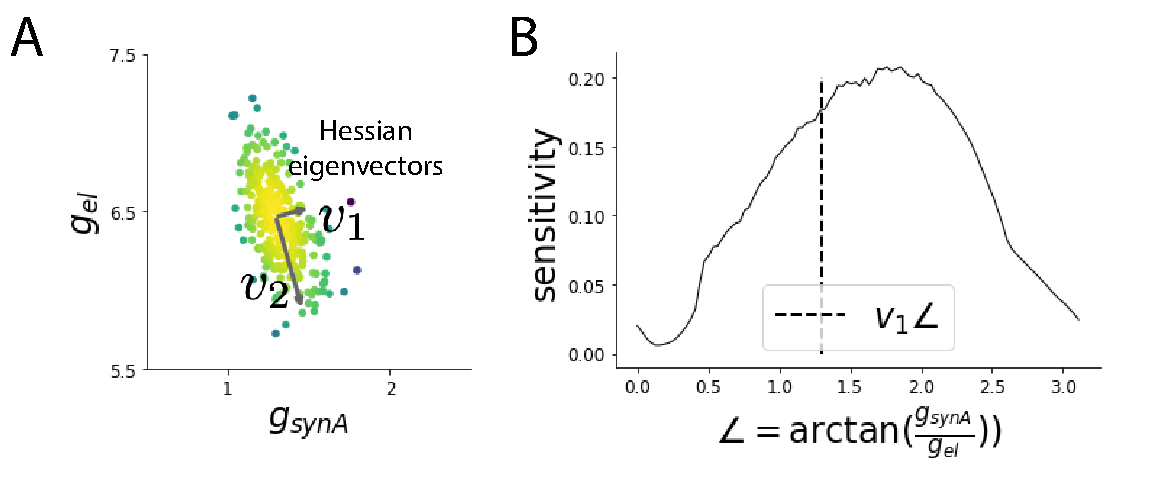
\includegraphics[scale=0.7]{figs/figS1/figS1.pdf}
\end{center}
Fig. S1: A. DSN distribution of STG model parameters producing network syncing.  B. Sensitivity of the system with respect to network syncing along all dimensions of parameter space away from the mode.
\end{figure}


\begin{figure}
\begin{center}
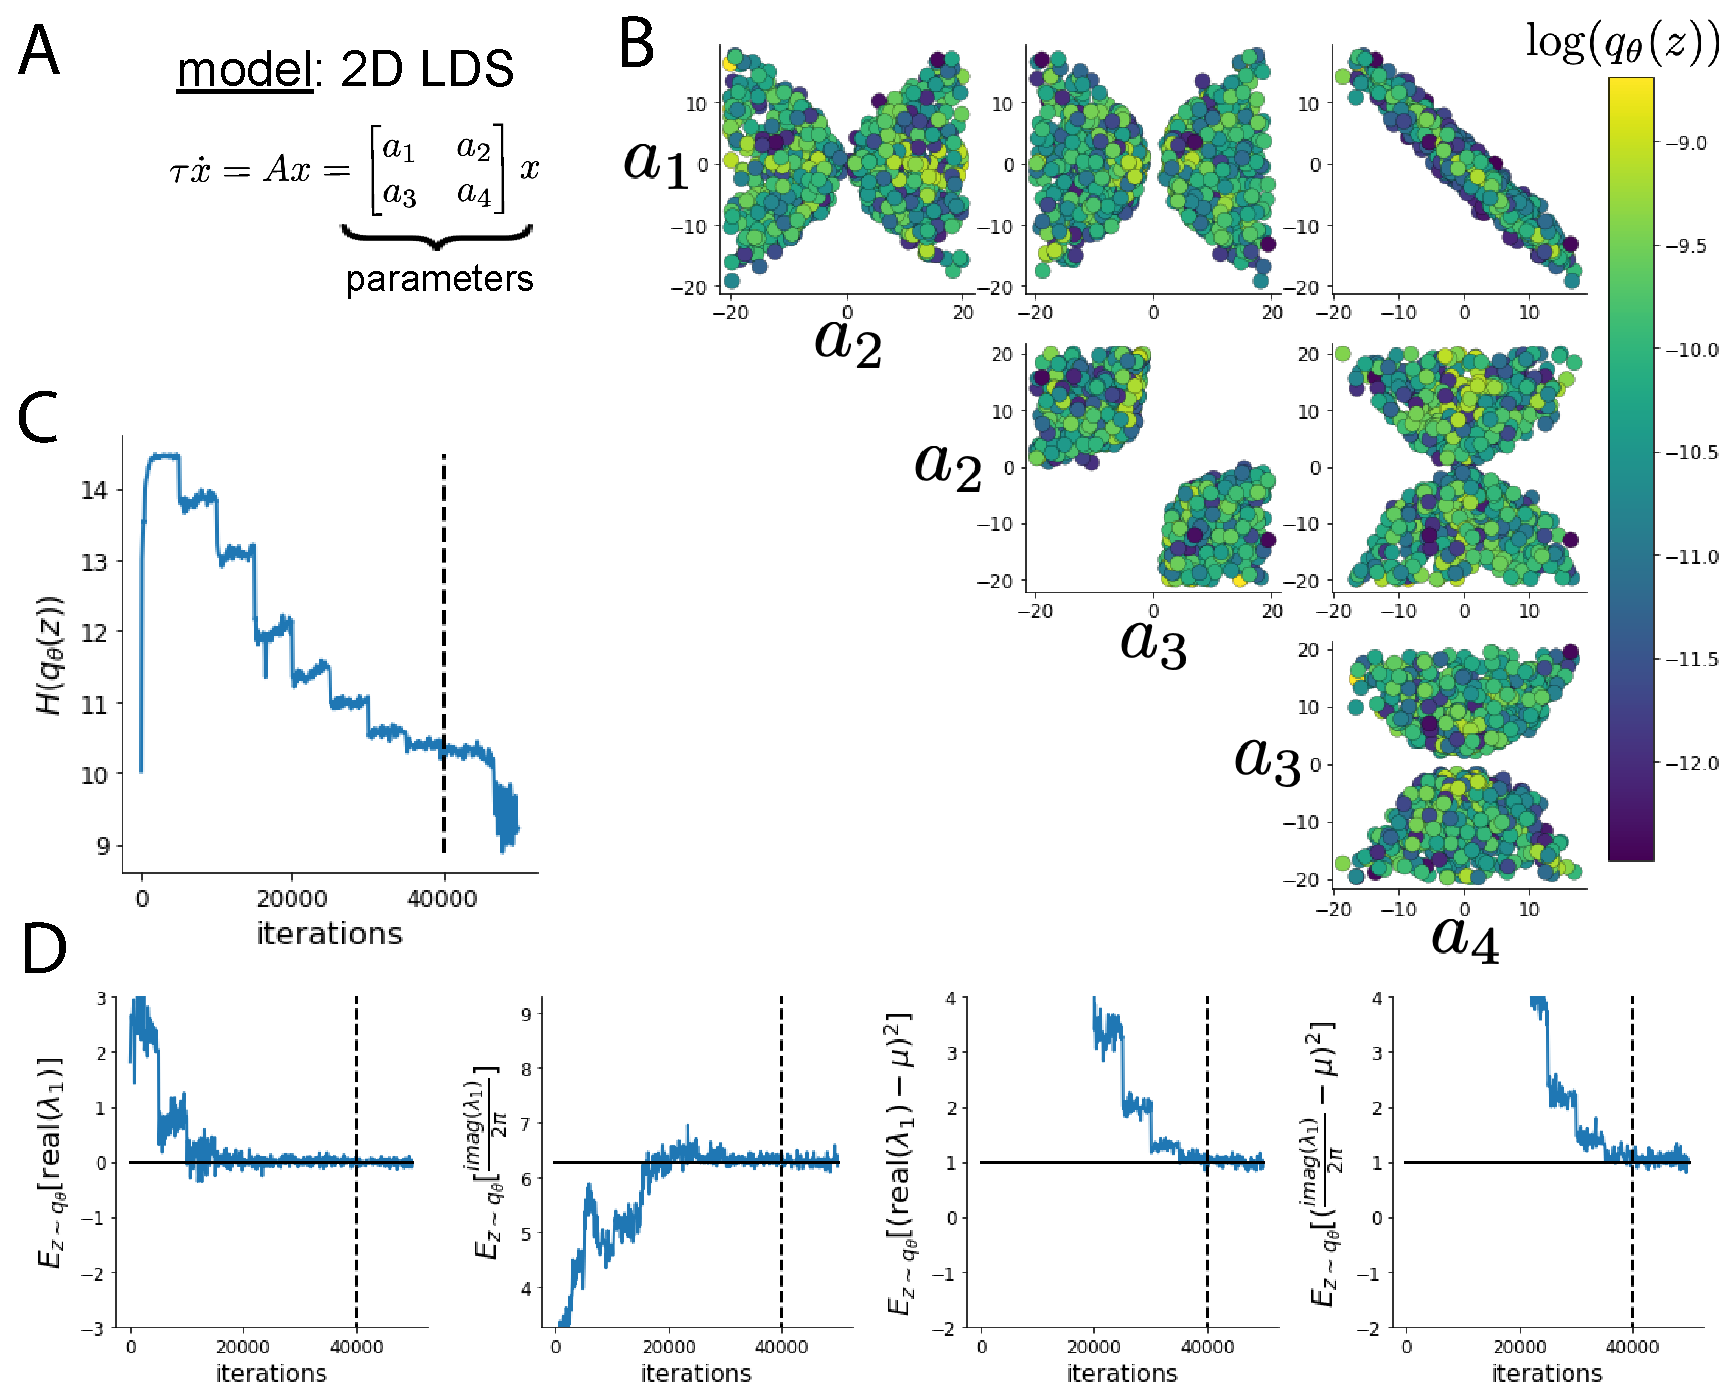
\includegraphics[scale=0.5]{figs/figS2/figS2.pdf}
\end{center}
Fig. S2: A. Two-dimensional linear dynamical system model, where real entries of the dynamics matrix $A$ are the parameters.  B. The DSN distribution for a 2D LDS with $\tau=1$ that produces an average of 1Hz oscillations with some small amount of variance.  C. Entropy throughout the optimization.  At the beginning of each augmented lagrangian epoch (5,000 iterations), the entropy dips due to the shifted optimization manifold where emergent property constraint satisfaction is increasingly weighted.  D. Emergent property moments throughout optimization.  At the beginning of each augmented lagrangian epoch, the emergent property moments move closer to their constraints.
\end{figure}




\bibliography{dsn}
\bibliographystyle{unsrt}

\end{document}


